\begin{frame} \frametitle{Сложные задачи}
	На «Математике НОН-СТОП» мы, разумеется, предлагаем задачи и для детей с некоторым опытом занятия в математических кружках — таким участникам также не будет скучно.
\end{frame}

\begin{frame} \frametitle{Девяносто десять}
\usl{7 класс, 4C}{Кого больше в двоичной записи чисел от 0 до $2^n - 1$ — единиц или нулей? Ответ объясните.} \vspace{4mm}

Нужно придумать однозначное соответствие между единицами \\
и нулями, в котором участвуют все нули, но не все единицы. \\
Но можно проще и изящнее: \ps

	Рассмотрим все возможные
	комбинации из $n$ нулей или единиц. В их записи, очевидно,
	встретится равное количество единиц и нулей. Чтобы получить
	записи чисел, отбросим все ведущие нули.
\end{frame}

\begin{frame} \frametitle{Карфаген\quad{\it\normalsize (Широкий не значит высокий)}}
\usl{8 класс, 1C}{Докажите, что максимальная возможная площадь $n$-угольника, все стороны которого имеют длину 1, меньше, чем максимальная возможная площадь $n+1$-угольника, все стороны которого имеют длину 1.} \vspace{4mm}

Дети же не знают, что максимальную площадь имеют \\
правильные $n$-угольники. \ps

Для каждого многоугольника с $n$ сторонами длины 1 построим многоугольник с $n+1$ сторонами, площадь которого больше.
\end{frame}

\begin{frame} \frametitle{Карфаген\quad{\it\normalsize (Широкий не значит высокий)}}

\begin{center}
\begin{tabular}{ccc}
Если выпуклый & & Если невыпуклый \\
\makecell[c]{
	\definecolor{carthfill}{RGB}{223,223,223}
	\tikz[scale=0.48]{
		\draw[thick] (-1,0) -- ++(60:2) -- (1,0) -- cycle;
		\filldraw[thick,fill=carthfill] (-1,0) ++(195:2) ++(210:2) --
		    ++(30:2) -- ++(15:2) -- ++(0:2) --
		    ++(-15:2) -- ++(-30:2);}
} & \hspace{0.6cm} &
\makecell[c]{
	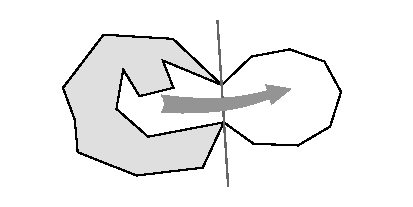
\includegraphics[scale=1.12]{img/carthage}
}
\end{tabular}\end{center}
\end{frame}

\begin{frame} \frametitle{Меняем правила под себя}

Рассмотрим следующую задачу, формулирующуюся \\
самым классическим образом: \medskip

\usl{8 класс, 10C}{В кучке $N$ камней. За ход из неё можно вынуть \vspace{-4mm}
	$$1,\ 2,\ 3,\ \ldots,\ a-1,\ \not{\!a},\ a+1,\ \ldots,\ n\text{\quad камней.}$$
	(То есть любое число от 1 до $n$, кроме $a$.) Играют двое, и про-\linebreak
	игрывает тот, кто не может сделать ход. Кто выиграет при правильной
	игре (в зависимости от чисел $N$, $n$, $a$)?}

Задача решается методом {\it анализа позиций:} не бывает ходов из проигрышной позиции в проигрышную.
\end{frame}

\begin{frame} \frametitle{Меняем правила под себя}
$a > \frac{n}{2}$: проигрышные позиции — $k \cdot a$. \ps
\begin{center} \tikz[scale=0.9]{
	\draw[thick,->] (-5,0) -- (5,0);
	\draw (-3,-0.24) -- (-3,0.24) (3,-0.24) -- (3,0.24);
	\draw (-3,-0.24) node[below]{$ka$} (3,-0.24) node[below]{$(k+1)a$};
	\draw[thick,->,color=red] (3,0.4) to[out=145,in=0]
		(0,1.35) node[above]{$a$} to[out=180,in=35] (-3,0.4);
	\draw[thick,->] (0.8,-0.27) to[out=225,in=0]
	(-1.2,-1.35) node[below]{$<a$} to[out=180,in=-30] (-3,-0.85);
} \end{center} \end{frame}

\definecolor{tturn}{RGB}{50,145,60}

\begin{frame} \frametitle{Меняем правила под себя}
$a \le \frac{n}{2}$: проигрышные позиции —
$k \cdot (n+a+1)$, $k \cdot (n+a+1) + a$. \medskip \\
Обозначим $s \coloneqq n+a+1$. \ps

\begin{center} \tikz[scale=0.92]{
	\draw[thick,->] (-7,0) -- (7,0);
	\foreach \x in {-5,-3.5,0,1.5,5} {\draw (\x,-0.18) -- (\x,0.18);}
	\draw (-5,-0.18) node[below]{$(k-1) \cdot s$}
		 (0,-0.18) node[below]{$k \cdot s$}
		 (5,-0.18) node[below]{$(k+1) \cdot s$}
		 (-3.5,0.18) node[above]{$+a$}
		 (1.5,0.18) node[above]{$+a$}
		 (-1.75,0) node[above]{\textcolor{red}{\footnotesize $n+1$}}
		 (3.25,0) node[above]{\textcolor{red}{\footnotesize $n+1$}};
	\draw[thick,color=tturn,->] (5,-0.8) to[out=215,in=-35] (1.5,-0.8);
	\draw[thick,color=tturn,->] (5,-0.8) to[out=215,in=-35] (0,-0.8);
	\draw[thick,color=tturn,->] (1.5,0.8) to[out=145,in=35] (-3.5,0.8);
	\draw[thick,color=tturn,->] (1.5,0.8) to[out=145,in=35] (-5,0.8);
} \end{center}
\end{frame}